\documentclass[10.5pt,a4paper]{article}
\usepackage[margin=1.45cm]{geometry}
\usepackage{amsmath,amssymb,mathtools}
\usepackage{booktabs,array,longtable,tabularx,multirow}
\usepackage{tikz}
\usetikzlibrary{arrows.meta,positioning,calc,shapes.geometric,trees}
\usepackage[most]{tcolorbox}
\usepackage{xcolor}
\usepackage{enumitem}
\usepackage{fancyhdr}
\usepackage{microtype}
\usepackage[T1]{fontenc}
\usepackage{lmodern}
\usepackage{hyperref}
\usepackage{listings}
\hypersetup{hidelinks}

\definecolor{primary}{HTML}{1F4E78}
\definecolor{qblue}{HTML}{EAF3FF}
\definecolor{ablue}{HTML}{EEF9F0}
\definecolor{qborder}{HTML}{2E75B6}
\definecolor{aborder}{HTML}{2E8B57}
\definecolor{noteorange}{HTML}{FFF4E5}
\definecolor{orangeborder}{HTML}{D98200}
\definecolor{deep}{HTML}{17365D}
\definecolor{graybox}{HTML}{F6F7F9}
\definecolor{softred}{HTML}{FDECEC}

\pagestyle{fancy}
\fancyhf{}
\lhead{CSE-3203: Design and Analysis of Algorithms-II}
\rhead{Final 2022 - Complete Q\&A Notes}
\cfoot{\thepage}
\setlength{\headheight}{14pt}

\newtcolorbox{questionbox}[2][]{
  enhanced, breakable,
  colback=qblue, colframe=qborder,
  boxrule=0.9pt, arc=1.5mm,
  title={\textbf{#2}}, fonttitle=\bfseries,
  coltitle=white, colbacktitle=qborder,
  attach boxed title to top left={xshift=2mm,yshift=-2mm},
  boxed title style={arc=1mm,boxrule=0pt},
  before skip=8pt, after skip=5pt,#1
}
\newtcolorbox{answerbox}[1][]{
  enhanced, breakable,
  colback=ablue, colframe=aborder,
  boxrule=0.8pt, arc=1.5mm,
  title={\textbf{Answer}}, fonttitle=\bfseries,
  coltitle=white, colbacktitle=aborder,
  attach boxed title to top left={xshift=2mm,yshift=-2mm},
  boxed title style={arc=1mm,boxrule=0pt},
  before skip=4pt, after skip=9pt,#1
}
\newtcolorbox{examtip}[1][]{
  enhanced, breakable,colback=noteorange,colframe=orangeborder,
  title={\textbf{Exam Tip}},fonttitle=\bfseries,coltitle=white,colbacktitle=orangeborder,
  boxrule=0.7pt,arc=1mm,#1
}
\newtcolorbox{keybox}[1][]{
  enhanced, breakable,colback=graybox,colframe=deep,
  title={\textbf{Key Result}},fonttitle=\bfseries,coltitle=white,colbacktitle=deep,
  boxrule=0.7pt,arc=1mm,#1
}
\newtcolorbox{warningbox}[1][]{
  enhanced,breakable,colback=softred,colframe=red!60!black,
  title={\textbf{Important Clarification}},fonttitle=\bfseries,coltitle=white,colbacktitle=red!60!black,
  boxrule=0.7pt,arc=1mm,#1
}

\lstset{basicstyle=\ttfamily\small,frame=single,breaklines=true,columns=fullflexible}
\setlist[itemize]{leftmargin=6mm}
\setlist[enumerate]{leftmargin=7mm}
\renewcommand{\arraystretch}{1.18}

\begin{document}

\begin{center}
{\LARGE\bfseries\color{primary} CSE-3203 Final Examination 2022}\par
\vspace{2mm}
{\Large\bfseries Design and Analysis of Algorithms-II}\par
\vspace{1mm}
{\large Complete Question \& Answer Notes}\par
\vspace{2mm}
{\small University of Dhaka, Department of Computer Science and Engineering}\par
\vspace{3mm}
\rule{0.9\textwidth}{0.6pt}
\end{center}

\begin{examtip}
The questions are transcribed from the two supplied exam-page screenshots. The answers are worked study solutions using standard algorithms from the course. Where a scan is slightly unclear, the interpretation used is stated explicitly.
\end{examtip}

\tableofcontents
\newpage

% =========================================================
\section{Question 1 - Hashing}

\begin{questionbox}{Q1(a) [4 marks]}
Describe the differences between \textbf{Linear Probing} and \textbf{Quadratic Probing} with proper examples.
\end{questionbox}

\begin{answerbox}
Both are open-addressing methods: all keys are stored inside the hash table and a probe sequence is used after a collision.

\begin{center}
\small
\begin{tabularx}{0.96\textwidth}{>{\bfseries}p{3cm}XX}
\toprule
Property & Linear probing & Quadratic probing\\
\midrule
Probe rule & $h(k,i)=(h'(k)+i)\bmod m$ & $h(k,i)=(h'(k)+c_1i+c_2i^2)\bmod m$; common simple form $h'(k)+i^2$\\
Step sizes & $1,1,1,\ldots$ & Increasing/nonlinear offsets\\
Clustering & Suffers from primary clustering & Avoids primary clustering, though secondary clustering may remain\\
Coverage & With unit step, all slots are eventually examined & Choice of $m,c_1,c_2$ matters; a poor choice may not visit every slot\\
Implementation & Very simple, cache friendly & Slightly more arithmetic\\
\bottomrule
\end{tabularx}
\end{center}

\textbf{Example.} Let $m=7$, $h'(k)=k\bmod7$, and insert $10,17,24$. All three initially hash to slot $3$.

Linear probing gives
\[
10\to3,\qquad17\to4,\qquad24\to5.
\]
Quadratic probing with $i^2$ gives
\[
10\to3,\qquad17\to(3+1^2)=4,
\]
and for $24$, slots $3$ and $4$ are occupied, so
\[
24\to(3+2^2)\bmod7=0.
\]
Thus quadratic probing spreads colliding keys more widely.
\end{answerbox}

\begin{questionbox}{Q1(b) [2 marks]}
The hash table has indices $0$ through $8$ and currently contains
\[
H[1]=11,\quad H[2]=101,\quad H[4]=22,\quad H[5]=50,\quad H[7]=34.
\]
For a new number $n$, its initial index is
\[
\text{idx}=n\bmod9.
\]
Identify which of the following entries creates a collision (multiple entries for the same index):
\[
600,\quad666,\quad682,\quad701.
\]
\end{questionbox}

\begin{answerbox}
Compute each initial index:
\[
600\bmod9=6,
\qquad
666\bmod9=0,
\]
\[
682\bmod9=7,
\qquad
701\bmod9=8.
\]
The only occupied one among these indices is index $7$, which already contains $34$. Therefore
\[
\boxed{682\text{ creates a collision at index }7.}
\]
The other three map to empty slots $6,0,8$.
\end{answerbox}

\begin{questionbox}{Q1(c) [8 marks]}
The scan gives the string
\[
S=\texttt{aaaaacbafadfcbb}.
\]
For every consecutive substring of length $3$, compute
\[
H_{i,i+2}
=
\bigl(\operatorname{ASCII}(S[i])B^2
+\operatorname{ASCII}(S[i+1])B
+\operatorname{ASCII}(S[i+2])\bigr)\bmod M,
\]
where $B=7$ and $M=13$. Identify whether two \emph{different} three-character sequences can have the same hash value.
\end{questionbox}

\begin{answerbox}
Here $B^2=49$. Evaluating every length-$3$ window gives:

\begin{center}
\small
\begin{tabular}{c c c@{\qquad}c c c}
\toprule
$i$ & substring & hash & $i$ & substring & hash\\
\midrule
0 & \texttt{aaa} & 4 & 7 & \texttt{afa} & 0\\
1 & \texttt{aaa} & 4 & 8 & \texttt{fad} & 5\\
2 & \texttt{aaa} & 4 & 9 & \texttt{adf} & 4\\
3 & \texttt{aac} & 6 & 10 & \texttt{dfc} & 6\\
4 & \texttt{acb} & 6 & 11 & \texttt{fcb} & 4\\
5 & \texttt{cba} & 5 & 12 & \texttt{cbb} & 6\\
6 & \texttt{baf} & 6 & & &\\
\bottomrule
\end{tabular}
\end{center}

The repeated \texttt{aaa} windows are the same sequence, so they are not a collision between different strings. But several \emph{different} triples share the same hash:
\[
\boxed{h=4:\ \texttt{aaa},\texttt{adf},\texttt{fcb}}
\]
\[
\boxed{h=5:\ \texttt{cba},\texttt{fad}}
\]
\[
\boxed{h=6:\ \texttt{aac},\texttt{acb},\texttt{baf},\texttt{dfc},\texttt{cbb}}
\]
Hence this hash function definitely has collisions.
\end{answerbox}

% =========================================================
\section{Question 2 - String Matching and Tries}

\begin{questionbox}{Q2(a) [4 marks]}
A pattern is called \textbf{nonoverlappable} when it has no nonempty proper prefix that is also a suffix. Give an example and describe the state-transition diagram of the string-matching automaton for a nonoverlappable pattern.
\end{questionbox}

\begin{answerbox}
A simple example is
\[
P=\texttt{ab}.
\]
Its only nonempty proper prefix is \texttt{a}, while its only length-$1$ suffix is \texttt{b}; hence they are different and the pattern cannot overlap with itself.

For alphabet $\Sigma=\{a,b\}$, the string-matching automaton has states $q_0,q_1,q_2$, where state $q$ means that the longest prefix of $P$ matching a suffix of the text read so far has length $q$. State $q_2$ is accepting.

\begin{center}
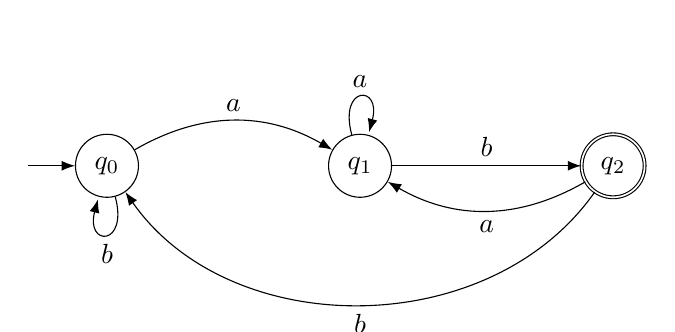
\begin{tikzpicture}[node distance=2.4cm,>=Latex]
\node[draw,circle,minimum size=8mm] (q0) {$q_0$};
\node[draw,circle,minimum size=8mm,right=of q0] (q1) {$q_1$};
\node[draw,double,circle,minimum size=8mm,right=of q1] (q2) {$q_2$};
\draw[->] (-1.0,0)--(q0);
\draw[->] (q0) edge[bend left] node[above] {$a$} (q1);
\draw[->] (q0) edge[loop below] node {$b$} (q0);
\draw[->] (q1) edge[loop above] node {$a$} (q1);
\draw[->] (q1) edge node[above] {$b$} (q2);
\draw[->] (q2) edge[bend left] node[below] {$a$} (q1);
\draw[->] (q2) edge[bend left=55] node[below] {$b$} (q0);
\end{tikzpicture}
\end{center}

Transition table:
\[
\begin{array}{c|cc}
 & a & b\\ \hline
\to q_0&q_1&q_0\\
q_1&q_1&q_2\\
* q_2&q_1&q_0
\end{array}
\]
The important nonoverlap property is that after a full match there is no positive-length border of the whole pattern to reuse.
\end{answerbox}

\begin{questionbox}{Q2(b) [4 marks]}
Draw a standard trie for
\[
\{\texttt{abab},\texttt{baba},\texttt{ccccc},\texttt{bbaaaa},\texttt{caa},\texttt{bbaacc},\texttt{cbcc},\texttt{cbca}\}.
\]
\end{questionbox}

\begin{answerbox}
A standard trie uses one character per edge. Green boxes mark complete words.

\begin{center}
\resizebox{0.96\textwidth}{!}{%
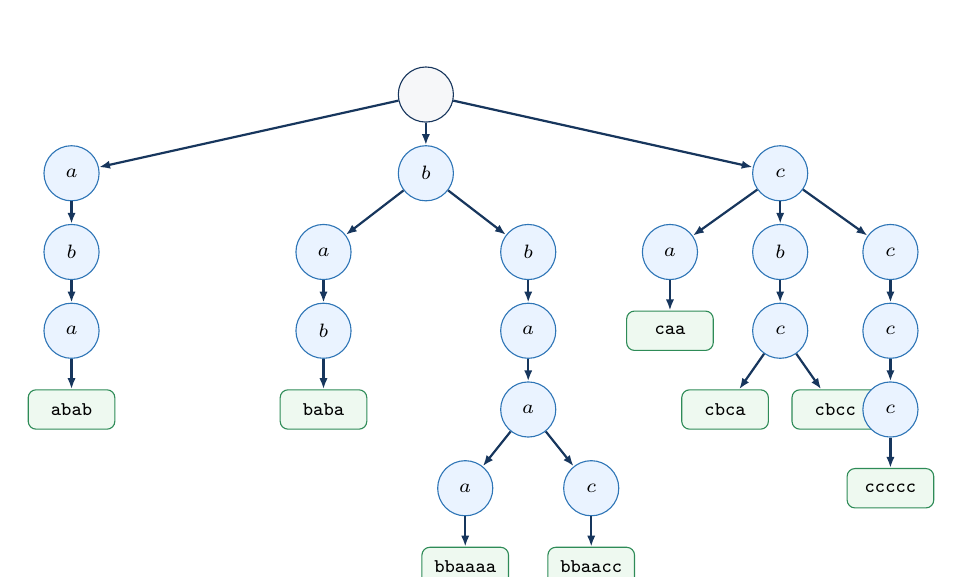
\begin{tikzpicture}[
 every node/.style={font=\scriptsize},
 root/.style={draw=deep,fill=graybox,circle,minimum size=7mm},
 node/.style={draw=qborder,fill=qblue,circle,minimum size=7mm},
 leaf/.style={draw=aborder,fill=ablue,rounded corners=1mm,minimum width=11mm,minimum height=5mm},
 edge/.style={-{Latex[length=1.4mm]},thick,draw=deep}
]
\node[root] (r) at (0,0) {};
\node[node] (a) at (-4.5,-1) {$a$};
\node[node] (b) at (0,-1) {$b$};
\node[node] (c) at (4.5,-1) {$c$};
\draw[edge] (r)--(a); \draw[edge] (r)--(b); \draw[edge] (r)--(c);

\node[node] (ab) at (-4.5,-2) {$b$};
\node[node] (aba) at (-4.5,-3) {$a$};
\node[leaf] (abab) at (-4.5,-4) {\texttt{abab}};
\draw[edge] (a)--(ab); \draw[edge] (ab)--(aba); \draw[edge] (aba)--(abab);

\node[node] (ba) at (-1.3,-2) {$a$};
\node[node] (bb) at (1.3,-2) {$b$};
\draw[edge] (b)--(ba); \draw[edge] (b)--(bb);
\node[node] (bab) at (-1.3,-3) {$b$};
\node[leaf] (baba) at (-1.3,-4) {\texttt{baba}};
\draw[edge] (ba)--(bab); \draw[edge] (bab)--(baba);
\node[node] (bba) at (1.3,-3) {$a$};
\node[node] (bbaa) at (1.3,-4) {$a$};
\node[node] (bbaaa) at (0.5,-5) {$a$};
\node[node] (bbaac) at (2.1,-5) {$c$};
\node[leaf] (bbaaaa) at (0.5,-6) {\texttt{bbaaaa}};
\node[leaf] (bbaacc) at (2.1,-6) {\texttt{bbaacc}};
\draw[edge] (bb)--(bba); \draw[edge] (bba)--(bbaa);
\draw[edge] (bbaa)--(bbaaa); \draw[edge] (bbaa)--(bbaac);
\draw[edge] (bbaaa)--(bbaaaa); \draw[edge] (bbaac)--(bbaacc);

\node[node] (ca) at (3.1,-2) {$a$};
\node[node] (cb) at (4.5,-2) {$b$};
\node[node] (cc) at (5.9,-2) {$c$};
\draw[edge] (c)--(ca); \draw[edge] (c)--(cb); \draw[edge] (c)--(cc);
\node[leaf] (caa) at (3.1,-3) {\texttt{caa}}; \draw[edge] (ca)--(caa);
\node[node] (cbc) at (4.5,-3) {$c$};
\node[leaf] (cbca) at (3.8,-4) {\texttt{cbca}};
\node[leaf] (cbcc) at (5.2,-4) {\texttt{cbcc}};
\draw[edge] (cb)--(cbc); \draw[edge] (cbc)--(cbca); \draw[edge] (cbc)--(cbcc);
\node[node] (ccc) at (5.9,-3) {$c$};
\node[node] (cccc) at (5.9,-4) {$c$};
\node[leaf] (ccccc) at (5.9,-5) {\texttt{ccccc}};
\draw[edge] (cc)--(ccc); \draw[edge] (ccc)--(cccc); \draw[edge] (cccc)--(ccccc);
\end{tikzpicture}}
\end{center}
\end{answerbox}

\begin{questionbox}{Q2(c) [6 marks]}
Given a string $X$ of length $n$ and a string $Y$ of length $m$, describe an $O(n+m)$-time algorithm for finding the longest prefix of $X$ that is a suffix of $Y$.
\end{questionbox}

\begin{answerbox}
Use the KMP prefix function on one combined string.

Choose a separator symbol $\#$ that occurs in neither string, and form
\[
Z=X\#Y.
\]
Compute the prefix function $\pi$ for $Z$ in linear time. The value at the last position,
\[
\boxed{\pi[|Z|]},
\]
is exactly the length of the longest prefix of $X$ that is also a suffix of $Y$.

Why it works: any prefix-suffix match at the end of $Z$ must start at the beginning of $X$. The separator prevents a match from crossing from the end of $X$ into the beginning of $Y$.

\begin{lstlisting}
LongestPrefixSuffix(X, Y):
    Z = X + "#" + Y
    pi = PrefixFunction(Z)
    L = pi[len(Z)-1]
    return X[0 : L]
\end{lstlisting}

Since $|Z|=n+m+1$ and KMP computes $\pi$ in linear time,
\[
\boxed{T(n,m)=O(n+m).}
\]
\end{answerbox}

% =========================================================
\section{Question 3 - Computational Geometry}

\begin{questionbox}{Q3(a) [3 marks]}
Prove that if $p_1\times p_2$ is positive, then vector $p_1$ is clockwise from vector $p_2$ with respect to the origin $(0,0)$, and if the cross product is negative, then $p_1$ is counterclockwise from $p_2$.
\end{questionbox}

\begin{answerbox}
Write the vectors in polar form:
\[
p_1=r_1(\cos\theta_1,\sin\theta_1),
\qquad
p_2=r_2(\cos\theta_2,\sin\theta_2).
\]
Then
\[
\begin{aligned}
p_1\times p_2
&=r_1r_2(\cos\theta_1\sin\theta_2-\sin\theta_1\cos\theta_2)\\
&=r_1r_2\sin(\theta_2-\theta_1).
\end{aligned}
\]
Because $r_1r_2>0$, the sign is determined by $\sin(\theta_2-\theta_1)$.

If $p_1\times p_2>0$, rotating counterclockwise from $p_1$ reaches $p_2$ through the smaller angle; equivalently $p_1$ is clockwise from $p_2$. If the cross product is negative, the relative orientation reverses. If it is zero, the vectors are collinear.

\begin{keybox}
For the ordering used in the question:
\[
\boxed{p_1\times p_2>0\Rightarrow p_1\text{ clockwise from }p_2}
\]
\[
\boxed{p_1\times p_2<0\Rightarrow p_1\text{ counterclockwise from }p_2.}
\]
\end{keybox}
\end{answerbox}

\begin{questionbox}{Q3(b) [6 marks]}
For the crossing segments shown, with $p_1$ upper-left, $p_2$ lower-right, $p_3$ lower-left and $p_4$ upper-right, determine whether each expression is positive or negative:
\[
\begin{array}{ll}
\text{i.}&(p_1-p_3)\times(p_4-p_3),\\
\text{ii.}&(p_3-p_1)\times(p_2-p_1),\\
\text{iii.}&(p_4-p_1)\times(p_2-p_1),\\
\text{iv.}&(p_2-p_3)\times(p_4-p_3).
\end{array}
\]
\end{questionbox}

\begin{answerbox}
Only the signs are needed, so we may use any coordinates preserving the drawing, for example
\[
p_1=(-1,1),\quad p_2=(1,-1),\quad p_3=(-1,-1),\quad p_4=(1,1).
\]
Then:
\[
(p_1-p_3)\times(p_4-p_3)
=(0,2)\times(2,2)=-4<0,
\]
\[
(p_3-p_1)\times(p_2-p_1)
=(0,-2)\times(2,-2)=4>0,
\]
\[
(p_4-p_1)\times(p_2-p_1)
=(2,0)\times(2,-2)=-4<0,
\]
\[
(p_2-p_3)\times(p_4-p_3)
=(2,0)\times(2,2)=4>0.
\]
Therefore
\[
\boxed{\text{i }<0,\qquad \text{ii }>0,\qquad \text{iii }<0,\qquad \text{iv }>0.}
\]
\end{answerbox}

\begin{questionbox}{Q3(c) [5 marks]}
Write the pseudocode of Graham Scan to generate a convex hull from a set of points. Show two cases (with diagram): (i) include a point as a hull vertex and (ii) exclude a point from the hull vertex set.
\end{questionbox}

\begin{answerbox}
\textbf{Graham Scan.}
\begin{lstlisting}
GRAHAM-SCAN(P):
    p0 = point with minimum y
         (break tie by minimum x)
    sort remaining points by increasing polar angle about p0
    for equal angles keep only the farthest point

    S = empty stack
    push p0
    push first sorted point
    push second sorted point

    for each remaining point p:
        while size(S) >= 2 and
              orientation(nextToTop(S), top(S), p) <= 0:
            pop(S)
        push(S, p)

    return S
\end{lstlisting}

Using the usual orientation
\[
\operatorname{orient}(A,B,C)=(B-A)\times(C-A),
\]
a positive value means a left turn.

\begin{center}
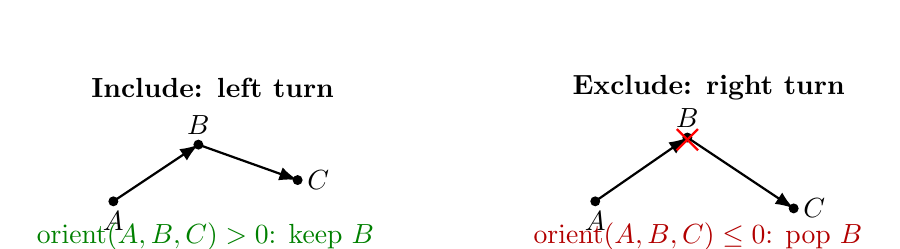
\begin{tikzpicture}[scale=0.9,>=Latex]
\node at (-3.6,1.6) {\bfseries Include: left turn};
\coordinate (A) at (-5,0); \coordinate (B) at (-3.8,0.8); \coordinate (C) at (-2.4,0.3);
\fill (A) circle (2pt) node[below] {$A$}; \fill (B) circle (2pt) node[above] {$B$}; \fill (C) circle (2pt) node[right] {$C$};
\draw[->,thick] (A)--(B); \draw[->,thick] (B)--(C);
\node[green!50!black] at (-3.7,-0.5) {$\operatorname{orient}(A,B,C)>0$: keep $B$};

\node at (3.4,1.6) {\bfseries Exclude: right turn};
\coordinate (D) at (1.8,0); \coordinate (E) at (3.1,0.9); \coordinate (F) at (4.6,-0.1);
\fill (D) circle (2pt) node[below] {$A$}; \fill (E) circle (2pt) node[above] {$B$}; \fill (F) circle (2pt) node[right] {$C$};
\draw[->,thick] (D)--(E); \draw[->,thick] (E)--(F);
\draw[red,thick] (2.95,0.72)--(3.25,1.02); \draw[red,thick] (2.95,1.02)--(3.25,0.72);
\node[red!70!black] at (3.25,-0.5) {$\operatorname{orient}(A,B,C)\le0$: pop $B$};
\end{tikzpicture}
\end{center}

Thus Graham Scan keeps points that preserve the counterclockwise boundary and removes points producing a right turn (or an unwanted collinear interior point).
\end{answerbox}

% =========================================================
\section{Question 4 - Number Theory and RSA}

\begin{questionbox}{Q4(a) [4 marks]}
Compute the values $d,x,y$ for $(899,493)$ using the Extended Euclidean Algorithm, where
\[
d=\gcd(899,493)=899x+493y.
\]
\end{questionbox}

\begin{answerbox}
Euclid's algorithm:
\[
899=1(493)+406,
\]
\[
493=1(406)+87,
\]
\[
406=4(87)+58,
\]
\[
87=1(58)+29,
\]
\[
58=2(29)+0.
\]
Hence
\[
\boxed{d=29}.
\]
Back-substitute:
\[
29=87-58
=87-(406-4\cdot87)
=5\cdot87-406,
\]
\[
=5(493-406)-406
=5\cdot493-6\cdot406,
\]
\[
=5\cdot493-6(899-493)
=11\cdot493-6\cdot899.
\]
Therefore
\[
\boxed{d=29,\qquad x=-6,\qquad y=11.}
\]
Check:
\[
899(-6)+493(11)=29.
\]
\end{answerbox}

\begin{questionbox}{Q4(b) [3 marks]}
Find Euler's totient function $\phi(7000)$.
\end{questionbox}

\begin{answerbox}
Factorise:
\[
7000=2^3\cdot5^3\cdot7.
\]
Then
\[
\phi(7000)
=7000\left(1-\frac12\right)
\left(1-\frac15\right)
\left(1-\frac17\right).
\]
Thus
\[
\phi(7000)=7000\cdot\frac12\cdot\frac45\cdot\frac67
=\boxed{2400}.
\]
\end{answerbox}

\begin{questionbox}{Q4(c) [7 marks]}
Consider an RSA key set with $p=17$, $q=11$, $n=187$, and $e=7$. Determine the public and private keys. What is the encryption of message $M=88$? Also prove by decryption that the recovered message is $88$.
\end{questionbox}

\begin{answerbox}
First,
\[
\phi(n)=(17-1)(11-1)=16\cdot10=160.
\]
The private exponent $d$ satisfies
\[
7d\equiv1\pmod{160}.
\]
Since
\[
7\cdot23=161\equiv1\pmod{160},
\]
we get
\[
\boxed{d=23}.
\]
Therefore:
\[
\boxed{\text{Public key }(e,n)=(7,187)}
\]
\[
\boxed{\text{Private key }(d,n)=(23,187)}.
\]

\textbf{Encryption.}
\[
C=M^e\bmod n=88^7\bmod187.
\]
Use repeated squaring:
\[
88^2\equiv77\pmod{187},
\qquad
88^4\equiv132\pmod{187}.
\]
Hence
\[
88^7=88^4\cdot88^2\cdot88
\equiv132\cdot77\cdot88
\equiv\boxed{11}\pmod{187}.
\]
So the ciphertext is $C=11$.

\textbf{Decryption.}
\[
M'=C^d\bmod n=11^{23}\bmod187.
\]
Now
\[
11^2\equiv121,
\quad11^4\equiv55,
\quad11^8\equiv33,
\quad11^{16}\equiv154\pmod{187}.
\]
Since $23=16+4+2+1$,
\[
11^{23}\equiv154\cdot55\cdot121\cdot11\equiv\boxed{88}\pmod{187}.
\]
Thus decryption recovers the original message.
\end{answerbox}

% =========================================================
\section{Question 5 - Backtracking and Branch and Bound}

\begin{questionbox}{Q5(a) [3 marks]}
Distinguish between backtracking and branch and bound.
\end{questionbox}

\begin{answerbox}
\begin{center}
\small
\begin{tabularx}{0.96\textwidth}{>{\bfseries}p{3.0cm}XX}
\toprule
Aspect & Backtracking & Branch and Bound\\
\midrule
Main goal & Find feasible/all solutions to constraint problems & Find an optimal solution to an optimisation problem\\
Pruning & Reject a partial solution that violates constraints or cannot become feasible & Reject a node whose bound cannot beat the current best solution\\
Typical search & Depth-first recursion & Best-first, BFS, or other live-node strategy\\
Main quantity & Promising/feasibility test & Lower or upper bound plus incumbent\\
Examples & N-Queens, subset sum, graph colouring, Hamiltonian cycle & 0/1 knapsack, TSP, assignment\\
Stopping & May stop after one feasible solution if only one is needed & Must establish that no live node can improve the incumbent\\
\bottomrule
\end{tabularx}
\end{center}

Memory rule:
\[
\boxed{\text{Backtracking prunes infeasible branches; B\&B also prunes noncompetitive branches.}}
\]
\end{answerbox}

\begin{questionbox}{Q5(b) [5 marks]}
Given the set
\[
S=\{5,10,12,13,15,18\}
\]
and target sum $m=30$, draw the state-space tree to print subsets whose sum equals $30$ using backtracking. Also define the bounding functions.
\end{questionbox}

\begin{answerbox}
Let the numbers be sorted increasingly. Use a binary decision at each level: include or exclude the next item.

A node stores
\[
(s,r),
\]
where $s$ is the current selected sum and $r$ is the sum of still-available elements. Initially
\[
(s,r)=(0,73).
\]

The three solution subsets are
\[
\boxed{\{5,10,15\}},\qquad
\boxed{\{5,12,13\}},\qquad
\boxed{\{12,18\}}.
\]
For example, one important branch is
\[
0\xrightarrow{+5}5\xrightarrow{+10}15\xrightarrow{-12}15
\xrightarrow{-13}15\xrightarrow{+15}\boxed{30}.
\]
Another is
\[
0\xrightarrow{+5}5\xrightarrow{-10}5\xrightarrow{+12}17
\xrightarrow{+13}\boxed{30},
\]
and the third is
\[
0\xrightarrow{-5}0\xrightarrow{-10}0\xrightarrow{+12}12
\xrightarrow{-13}12\xrightarrow{-15}12\xrightarrow{+18}\boxed{30}.
\]

\textbf{Bounding/promising conditions.} For current sum $s$, next item $w_{k+1}$, and total remaining sum $r$:
\[
\boxed{s+r\ge m}
\]
is necessary; otherwise even taking everything left cannot reach the target.

Also, for the next inclusion branch,
\[
\boxed{s+w_{k+1}\le m}
\]
must hold; otherwise the next inclusion already overshoots the target.

A standard recursive form is:
\begin{lstlisting}
SubsetSum(s, k, r):
    if s == m:
        print current subset
        return
    if k == n:
        return
    if s + r < m:
        return

    if s + w[k] <= m:
        choose w[k]
        SubsetSum(s + w[k], k+1, r - w[k])
        unchoose w[k]

    SubsetSum(s, k+1, r - w[k])
\end{lstlisting}
Branches with $s>30$ or $s+r<30$ are pruned.
\end{answerbox}

\begin{questionbox}{Q5(c) [6 marks]}
For the 0/1-knapsack instance below with capacity $W=10$ kg, compare backtracking and branch and bound by their state-space trees.

\begin{center}
\begin{tabular}{c c c}
\toprule
Item & Weight & Profit\\
\midrule
A&2&40\\
B&3.14&50\\
C&1.98&100\\
D&5&95\\
E&3&30\\
\bottomrule
\end{tabular}
\end{center}
\end{questionbox}

\begin{answerbox}
The optimal subset is
\[
\boxed{\{A,C,D\}}
\]
with
\[
\text{weight}=2+1.98+5=8.98\le10,
\]
\[
\text{profit}=40+100+95=\boxed{235}.
\]

\begin{warningbox}
The exam scan appears to say ``prove that backtracking does better than branch and bound.'' For this standard knapsack example, the intended textbook point is the opposite: branch and bound can prune more than simple feasibility-only backtracking because it uses an optimistic profit bound. The same numerical instance is commonly used to illustrate this improvement. The solution below follows the standard algorithmic interpretation.
\end{warningbox}

\textbf{Backtracking tree idea.} In the original item order $A,B,C,D,E$, a feasibility-only DFS can prune only when weight exceeds $10$. Many feasible but low-profit nodes must still be explored because feasibility alone does not prove that they cannot beat the optimum.

\begin{center}
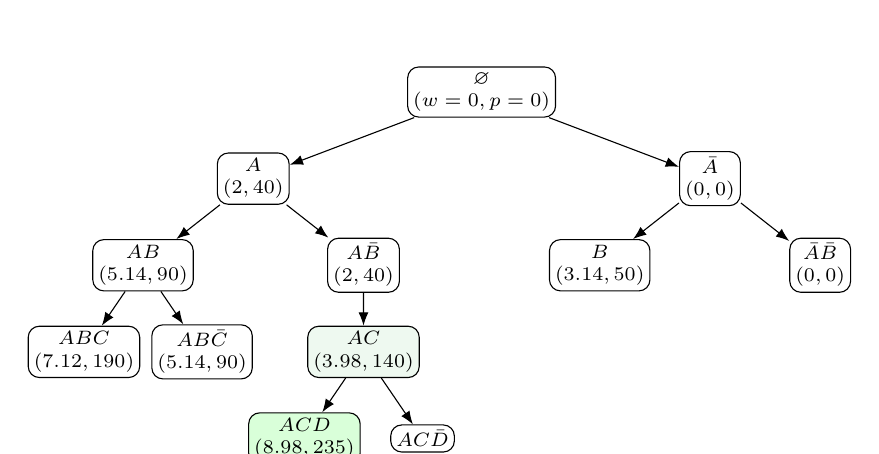
\begin{tikzpicture}[level distance=11mm,
level 1/.style={sibling distance=58mm},level 2/.style={sibling distance=28mm},level 3/.style={sibling distance=15mm},
every node/.style={draw,rounded corners,inner sep=2pt,font=\scriptsize,align=center},edge from parent/.style={draw,-Latex}]
\node {$\varnothing$\\$(w=0,p=0)$}
 child {node {$A$\\$(2,40)$}
   child {node {$AB$\\$(5.14,90)$}
     child {node {$ABC$\\$(7.12,190)$}}
     child {node {$AB\bar C$\\$(5.14,90)$}}
   }
   child {node {$A\bar B$\\$(2,40)$}
     child {node[fill=ablue] {$AC$\\$(3.98,140)$}
       child {node[fill=green!15] {$ACD$\\$(8.98,235)$}}
       child {node {$AC\bar D$}}
     }
   }
 }
 child {node {$\bar A$\\$(0,0)$}
   child {node {$B$\\$(3.14,50)$}}
   child {node {$\bar A\bar B$\\$(0,0)$}}
 };
\end{tikzpicture}
\end{center}
The omitted descendants are still numerous; a branch is killed immediately only when its accumulated weight exceeds $10$.

\medskip
\textbf{Branch-and-bound tree.} First sort by profit/weight ratio:
\[
C\;(50.51),\quad A\;(20),\quad D\;(19),\quad B\;(15.92),\quad E\;(10).
\]
At each node use the fractional-knapsack value as an upper bound $UB$. A compact best-first tree is:

\begin{center}
\resizebox{0.98\textwidth}{!}{%
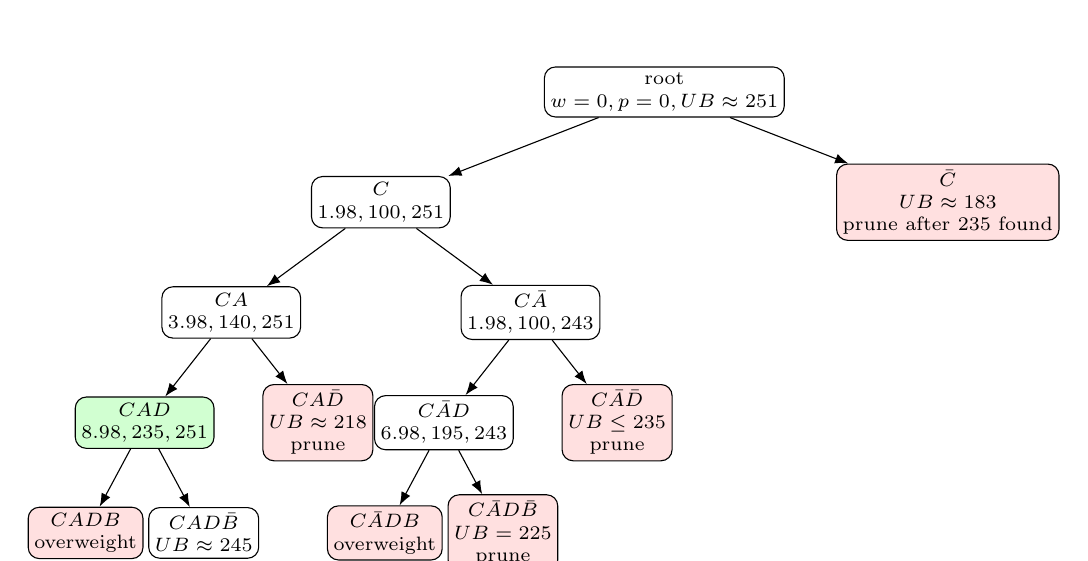
\begin{tikzpicture}[level distance=14mm,
level 1/.style={sibling distance=72mm},level 2/.style={sibling distance=38mm},level 3/.style={sibling distance=22mm},level 4/.style={sibling distance=15mm},
every node/.style={draw,rounded corners,inner sep=2.2pt,font=\scriptsize,align=center},edge from parent/.style={draw,-Latex}]
\node {root\\$w=0,p=0,UB\approx251$}
 child {node {$C$\\$1.98,100,251$}
   child {node {$CA$\\$3.98,140,251$}
     child {node[fill=green!18] {$CAD$\\$8.98,235,251$}
       child {node[fill=red!12] {$CADB$\\overweight}}
       child {node {$CAD\bar B$\\$UB\approx245$}}
     }
     child {node[fill=red!12] {$CA\bar D$\\$UB\approx218$\\prune}}
   }
   child {node {$C\bar A$\\$1.98,100,243$}
     child {node {$C\bar AD$\\$6.98,195,243$}
       child {node[fill=red!12] {$C\bar ADB$\\overweight}}
       child {node[fill=red!12] {$C\bar AD\bar B$\\$UB=225$\\prune}}
     }
     child {node[fill=red!12] {$C\bar A\bar D$\\$UB\le235$\\prune}}
   }
 }
 child {node[fill=red!12] {$\bar C$\\$UB\approx183$\\prune after $235$ found}};
\end{tikzpicture}}
\end{center}

Once profit $235$ is found, every live node with $UB\le235$ is discarded. This extra bound-based pruning is exactly what branch and bound adds beyond plain backtracking.
\end{answerbox}

% =========================================================
\section{Question 6 - NP Problems, Reductions, and Circle Geometry}

\begin{questionbox}{Q6(a) [4 marks]}
Discuss the steps that are used to solve/prove a problem as an NP problem.
\end{questionbox}

\begin{answerbox}
The standard exam interpretation is the workflow for establishing NP-completeness.

\begin{enumerate}
\item \textbf{Write the decision version.} State clearly what constitutes a YES instance.
\item \textbf{Show membership in NP.} Give a certificate and a polynomial-time verifier.
\item \textbf{Choose a known NP-complete problem $A$.}
\item \textbf{Construct a polynomial reduction} $A\le_p B$, where $B$ is the new problem.
\item \textbf{Prove correctness of the reduction:}
\[
x\in A\iff f(x)\in B.
\]
\item Conclude that $B$ is NP-hard; together with $B\in NP$, conclude
\[
\boxed{B\text{ is NP-complete}.}
\]
\end{enumerate}
\end{answerbox}

\begin{questionbox}{Q6(b) [3 marks]}
Discuss the idea of a polynomial reduction algorithm to convert problem $A$ to another problem $B$.
\end{questionbox}

\begin{answerbox}
A polynomial-time reduction from $A$ to $B$, written
\[
A\le_p B,
\]
is an algorithm $f$ computable in polynomial time such that
\[
\boxed{x\in A\iff f(x)\in B.}
\]
To solve an instance $x$ of $A$ using a solver for $B$:
\[
\boxed{x\xrightarrow{\text{poly-time }f}f(x)\xrightarrow{\text{solve }B}\text{answer for }A.}
\]
Therefore, if
\[
A\le_p B
\quad\text{and}\quad
B\in P,
\]
then
\[
\boxed{A\in P.}
\]
For an NP-hardness proof, the direction is crucial: reduce a \emph{known hard problem} $A$ to the target $B$, not the other way around.
\end{answerbox}

\begin{questionbox}{Q6(c) [7 marks]}
Two circles are given as
\[
A=(A_x,A_y,A_r),\qquad B=(B_x,B_y,B_r),
\]
where the first two values are center coordinates and the last value is the radius. Write:
\begin{enumerate}[label=(\roman*)]
\item an algorithm to determine whether circles $A$ and $B$ intersect;
\item an algorithm to determine whether one circle lies inside the other.
\end{enumerate}
\end{questionbox}

\begin{answerbox}
Let
\[
d^2=(A_x-B_x)^2+(A_y-B_y)^2.
\]
Using squared distances avoids computing a square root.

\textbf{(i) Circumference intersection.} Two circles meet (including tangency) exactly when
\[
|A_r-B_r|\le d\le A_r+B_r.
\]
Equivalently,
\[
\boxed{(A_r-B_r)^2\le d^2\le(A_r+B_r)^2.}
\]

\begin{lstlisting}
CircleIntersect(A, B):
    d2 = (Ax-Bx)^2 + (Ay-By)^2
    return (Ar-Br)^2 <= d2 and d2 <= (Ar+Br)^2
\end{lstlisting}

\textbf{(ii) One circle inside the other.}
Circle $A$ is inside $B$ exactly when
\[
d+A_r\le B_r.
\]
For a square-root-free test, first require $B_r\ge A_r$, then test
\[
\boxed{d^2\le(B_r-A_r)^2.}
\]
Similarly, $B$ is inside $A$ if $A_r\ge B_r$ and
\[
d^2\le(A_r-B_r)^2.
\]

\begin{lstlisting}
Inside(A, B):
    d2 = (Ax-Bx)^2 + (Ay-By)^2
    if Br >= Ar and d2 <= (Br-Ar)^2:
        return "A inside B"
    if Ar >= Br and d2 <= (Ar-Br)^2:
        return "B inside A"
    return "neither contains the other"
\end{lstlisting}
Each algorithm uses only a constant number of arithmetic operations, so the running time is $O(1)$.
\end{answerbox}

% =========================================================
\section{Question 7 - Online Algorithms and List Update}

\begin{questionbox}{Q7(a) [3 marks]}
Mention the features of an online algorithm. Define the competitive ratio.
\end{questionbox}

\begin{answerbox}
An \textbf{online algorithm} receives requests one at a time and must make each decision without knowing future requests.

Important features:
\begin{itemize}
\item input arrives sequentially;
\item decisions are made immediately/irrevocably using only past and present information;
\item future input is unavailable;
\item performance is compared with an optimal offline algorithm $OPT$ that knows the full request sequence;
\item worst-case analysis is commonly used.
\end{itemize}

For a minimisation problem, algorithm $A$ is $c$-competitive if there exists a constant $\alpha$ such that for every request sequence $\sigma$,
\[
\boxed{A(\sigma)\le c\,OPT(\sigma)+\alpha.}
\]
Ignoring the additive constant for a long sequence, the competitive ratio is the worst-case ratio
\[
\boxed{\sup_{\sigma}\frac{A(\sigma)}{OPT(\sigma)}.}
\]
Smaller is better; $1$ would match the offline optimum.
\end{answerbox}

\begin{questionbox}{Q7(b) [11 marks]}
In the online list-update problem, the access cost of an item is proportional to its distance from the head of a linked list. Initially
\[
\Gamma=(1,2,3,\ldots,n),
\]
and requests arrive as $i_1,i_2,i_3,\ldots$. After an access, consider a strategy that moves the accessed item forward in the list.

\begin{enumerate}[label=(\roman*)]
\item Calculate/analyse the competitive ratio for the strategy that moves the accessed item forward by two positions.
\item Prove that no deterministic online list-update algorithm has a competitive ratio better than $2$ (asymptotically).
\end{enumerate}
\end{questionbox}

\begin{answerbox}
\textbf{(i) Move-Ahead-Two is not constant-competitive.}

Let the last three items initially be
\[
a=n-2,\qquad b=n-1,\qquad c=n.
\]
Use the repeating adversarial sequence
\[
\sigma=(c,b,a,c,b,a,\ldots).
\]
Initially the tail block is
\[
[a,b,c].
\]
Request $c$: it is at position $n$, costs $n$, and moving it forward two positions changes the tail block to
\[
[c,a,b].
\]
Next request $b$: again it is at position $n$, costs $n$, and the tail becomes
\[
[b,c,a].
\]
Next request $a$: again cost $n$, and the tail returns to
\[
[a,b,c].
\]
Thus this repeats forever, so Move-Ahead-Two pays approximately
\[
A(\sigma)=n\cdot |\sigma|.
\]
An offline optimum, knowing that only $a,b,c$ are repeatedly requested, can keep them in the first three positions; after an initial rearrangement its access cost is at most $3$ per request. Hence for a long sequence
\[
\frac{A(\sigma)}{OPT(\sigma)}\gtrsim\frac n3.
\]
Therefore
\[
\boxed{\text{Move-Ahead-Two has }\Omega(n)\text{ competitive ratio and is not constant-competitive}.}
\]

\medskip
\textbf{(ii) Deterministic lower bound approaching $2$.}

Consider any deterministic online algorithm $A$. An adversary repeatedly requests the item currently at the \emph{last} position of $A$'s list. Therefore $A$ pays
\[
n
\]
for every request. For a sequence of $m$ requests,
\[
A(\sigma)=mn.
\]

Now compare with a fixed offline ordering. If we choose a uniformly random permutation of the $n$ items, every requested item has expected position
\[
\frac{n+1}{2}.
\]
Therefore, by averaging, there exists at least one fixed ordering whose total cost on the same request sequence is at most
\[
\frac{m(n+1)}2.
\]
The true offline optimum can only be better, apart from an additive initial rearrangement cost. Hence, for long sequences,
\[
\frac{A(\sigma)}{OPT(\sigma)}
\ge
\frac{mn}{m(n+1)/2}
=
\frac{2n}{n+1}
=2-\frac{2}{n+1}.
\]
As $n\to\infty$,
\[
\frac{2n}{n+1}\to2.
\]
Thus no deterministic online algorithm can guarantee a competitive ratio strictly below $2$ for all list sizes:
\[
\boxed{\text{deterministic lower bound }=2\text{ asymptotically}.}
\]
\end{answerbox}

% =========================================================
\newpage
\section*{Last-Minute Revision Sheet}
\addcontentsline{toc}{section}{Last-Minute Revision Sheet}

\begin{center}
\small
\begin{tabularx}{0.98\textwidth}{>{\bfseries}p{3.2cm}X}
\toprule
Topic & Must remember\\
\midrule
Linear probing & $h(k,i)=(h'(k)+i)\bmod m$; primary clustering\\
Quadratic probing & $h(k,i)=(h'(k)+c_1i+c_2i^2)\bmod m$; reduces primary clustering\\
Hash collision Q1(b) & $682\bmod9=7$; index $7$ already occupied\\
Rolling hash Q1(c) & Distinct triples collide at hashes $4,5,6$\\
Nonoverlappable pattern & No nonempty proper prefix is also a suffix\\
Longest prefix of $X$ / suffix of $Y$ & Compute prefix function of $X\#Y$; answer is final $\pi$ value\\
Cross product & Sign gives relative orientation; Q3(b): $-,+,-,+$\\
Graham Scan & Sort by polar angle; pop while turn is non-left\\
Extended Euclid & $(899,493)\to(d,x,y)=(29,-6,11)$\\
Totient & $\phi(7000)=2400$\\
RSA & $(e,n)=(7,187)$, $(d,n)=(23,187)$, $88\to11\to88$\\
Subset Sum & Bounds: $s+r\ge m$ and next inclusion must not overshoot\\
Knapsack & Optimum $\{A,C,D\}$, weight $8.98$, profit $235$\\
NP-complete proof & In NP + known NP-C reduction $A\le_p B$ + iff correctness\\
Circle intersection & $(r_A-r_B)^2\le d^2\le(r_A+r_B)^2$\\
Online algorithm & No future knowledge; compare against offline $OPT$\\
Competitive ratio & $A(\sigma)\le cOPT(\sigma)+\alpha$\\
Move-Ahead-Two & Adversarial last-three cycle gives $\Omega(n)$ ratio\\
List-update lower bound & No deterministic algorithm beats $2$ asymptotically\\
\bottomrule
\end{tabularx}
\end{center}

\end{document}
